\chapter{Návrhové vzory Flux a Redux}

\label{kap:vzory} % id kapitoly pre prikaz ref

V tejto kapitole si povieme niečo o návrhových vzoroch Flux a Redux, ktoré sú určené na spracovávanie udalostí v aplikácii.

\section{Flux}
Hlavné črty návrhového vzoru Flux. \cite[Overview]{Flux} \TODO{}

Flux je vzor pre spravovanie dát v aplikácii. Najdôležitejším konceptom je tok informácií jedným smerom. Obsahuje štyri základné časti. 
\begin{itemize}
\item \emph{Akcie}, ktoré vytvára používateľ, prostredie, kde aplikácia beží alebo aj časti aplikácie. 
\item \emph{Dispečer} spravuje všetky vytvorené \emph{akcie}. 
\item \emph{Store} reaguje na \emph{akcie} a spravuje stav aplikácie.
\item \emph{View} ktorý vykresľuje stav aplikácie.
\end{itemize}
%TODO odkaz na obrazok

\subsection{Tok dát}%TODO skontroluj
\begin{enumerate}
\item daný úvodný stav
\item vykreslenie \emph{view} komponentov
\item vznik \emph{akcie}, oznámenie \emph{akcie} dispečeru (funkcia \emph{dispatch})
\item dispečer upozorní všetky \emph{story}
\item každý \emph{store} spracuje \emph{akciu}, prípadne zmení stav
\item zmena v stave sa vykreslí do komponentov (2. bod)
\end{enumerate}

%TODO zdroj
% zdroj: https://facebook.github.io/flux/img/flux-simple-f8-diagram-with-client-action-1300w.png

\begin{figure}
  \centering
    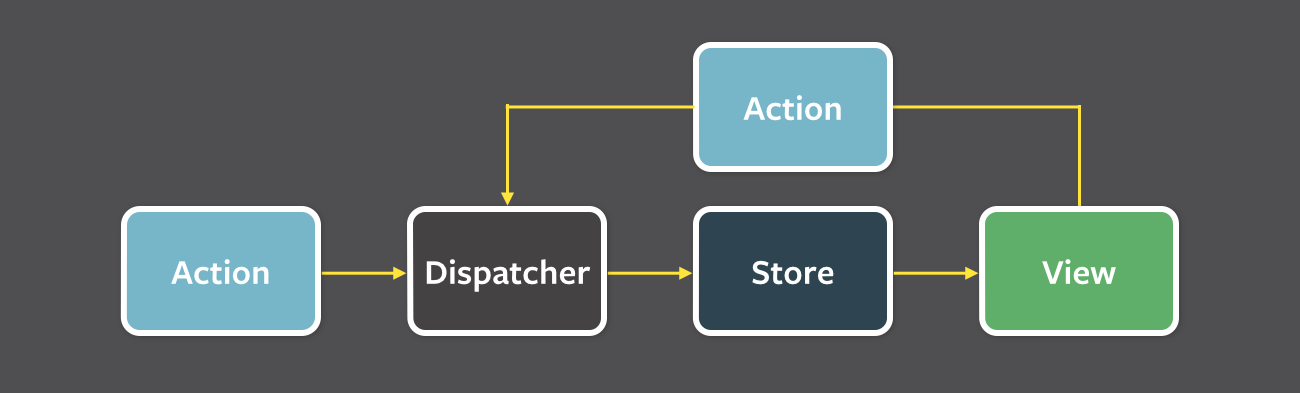
\includegraphics[width=\textwidth]{./images/flux.png}
  \caption{Flux architektúra}
\end{figure}

\subsection{Dispečer (dispatcher)}
Dispečer spravuje všetky akcie vykonané v aplikácii. V celej aplikácii by mal byť len jeden. Dispečer obsahuje spätné volanie (callback) na každý store v aplikácii. Keď sa vykoná nová akcia, dispečer pošle túto akciu všetkým storom. Sám nemusí obsahovať akúkoľvek vyššiu logiku, slúži len na distribúciu.

\subsection{Store}
Story obsahujú stav a logiku aplikácie. Store reaguje na akciu, na základe ktorej môže zmeniť stav, ktorý spravuje. Storov môže byť viac a každý upravuje nejakú podčasť dát. Každý store poskytuje dispečerovi na seba callback. Keď sa udeje nejaká akcia, bude o tom upozornený. Na základe typu akcie sa rozhodne, či a ako bude meniť stav aplikácie. (Napríklad ak máme dva story Images a Texts, tak pri vytvorení akcie EditText sa pravdepodobne store Image rozhodne nič nerobiť.) Po zmene stavu vytvorí udalosť, ktorou upozorní view časť, že treba prekresliť údaje.

\subsection{Akcie}
Akcie definujú internú API aplikácie. Zachytávajú možnosti interakcie s aplikáciou. Sú to jednoduché objekty s kľúčom \emph{typ} a voliteľnými pridanými informáciami. Typ akcie by nemal obsahovať žiadne implementačné detaily.

Akcie vytvára view časť (napríklad keď reagujeme na stlačenie tlačidla), server (napríklad chybová hláška počas komunikácie) alebo aj store (keď odstránime používateľa, chceme odstrániť aj všetky jeho príspevky).

\begin{lstlisting}[caption=Akcia vo Flux architektúre]
  {
  	type: 'delete-user',
  	userId: '1'
  }
\end{lstlisting}

\subsection{Views}
View je časť návrhu, ktorá vykresľuje stav zo storu. Aby bola táto časť vždy aktuálna, musí daný view komponent počúvať na všetky udalosti od storu, ktoré hovoria o zmene relevantných dát. Ak sa zmení stav, store vytvorí udalosť a view sa prekreslí. Architektúra flux neurčuje, ako má byť tento stav vykreslený.

\subsection{side effects} 
\TODO











\section{Redux}
Hlavné črty návrhového vzoru Redux. 

Redux je popis spracovania udalostí v aplikácii. Dáva do popredia lieárne spracovanie udalosti. Pozostáva zo štyroch hlavných častí:
\begin{itemize}
\item jeden \emph{store}, ktorý spravuje celý stav aplikácie
\item \emph{reducer} - čistá funkcia, ktorá jediná mení stav aplikácie
\item \emph{komponenty} vykresľujú aktuálny stav aplikácie
\item \emph{akcie}, ktoré definujú vnútorné rozhranie aplikácie
\end{itemize}

\subsection{Tok dát}
\begin{enumerate}
\item daný úvodný stav
\item vykreslenie \emph{komponentov}
\item vznik \emph{akcie}, dispečnutie akcie pre \emph{store}
\item \emph{reducer} na \emph{akcii} a aktuálnom stave, ktorý vráti nový stav
\item zmena v dátach sa vykreslí do \emph{komponentov} (2. bod)
\end{enumerate}

%TODO obrázok
%https://image.slidesharecdn.com/reactreduxintroduction-151124165017-lva1-app6891/95/react-redux-introduction-33-638.jpg?cb=1448383914
%https://www.slideshare.net/nikgraf/react-redux-introduction

\begin{figure}
  \centering
    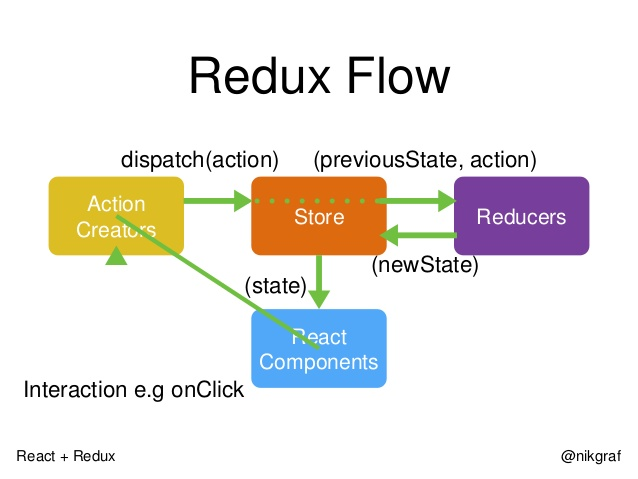
\includegraphics[width=0.8\textwidth]{./images/redux.jpg}
  \caption{Redux architektúra}
\end{figure}

\subsection{Store}
Store, správca stavu, vystupuje ako jediný zdroj pravdy v aplikácii. Všetky dáta, ktoré sú vykreslené, pochádzajú zo stavu. Teda ak poznáme tento stav, veľmi jednoducho vieme zostrojiť prostredie, v ktorom celá aplikácia beží. Rovnako v prípade chýb vieme oveľa jednoduchšie zistiť, kde chyba nastala. Tento stav je nemenný(immutable). Ak ho chceme zmeniť, musíme vytvoriť novú inštanciu, v ktorej urobíme potrebné zmeny.

Store má svoju funkciu \emph{dispatch()} ktorá slúži na vytváranie akcií. Všetky akcie by mali byť spracované cez túto funkciu. Na tieto akcie môže store reagovať zmenou stavu.

\subsection{Komponenty}
Komponenty slúžia na vykreslenie stavu aplikácie pre používateľa. Ponúkajú rozhranie pre používateľa na komunikáciu s programom. Komponenty vieme rozdeliť na stavové (\emph{Container Components}) a prezentačné (\emph{Presentational Components}).

Prezentačné komponenty iba vykresľujú data, ktoré dostanú. Starajú sa o výzor aplikácie. Tieto možno používať na viacerých miestach (nadpis, tabuľka). 

Stavové komponenty počúvajú na zmenu stavu. Majú na starosti, ako by mala stránka fungovať. V reduxovej aplikácii poskytujú rozhranie pre vytváranie akcií a majú prístup ku funkcii dispatch.

\subsection{Akcie}
Akcia je akákoľvek udalosť, ktorá sa môže v aplikácii vyskytnúť, od stlačenia tlačidla používateľom, až po chybové hlášky alebo stiahnutie dát zo servera. Na vytvorenie akcie používame funkciu dispatch. Každá akcia musí obsahovať typ a môže voliteľne obsahovať aj nejaké prídavné data. Na základe tejto akcie potom reducer vypočíta nový stav.

\subsection{Reducer}%TODO nie všetká, okrem toho sú aj side effects!
Takmer všetká logika aplikácie sa deje v reduceroch. Reducery sú jediný objekt, ktorý môže meniť stav aplikácie.

Reducer je čistá funkcia. Má dva argumenty, stav aplikácie a akciu, ktorá sa uskutočnila. Výstupom je nový stav. Vďaka vlastnosti, že nemá žiadne vedľajšie efekty, ju môžeme veľmi ľahko testovať.

Reducer môžeme vyskladať z viacerých menších čistých funkcií, kde každá z nich sa stará len o určitú malú časť stavu. Vďaka tomu zostáva kód prehľadný a jednoduchý. 
% nejaḱe kecy o funkcionalnom programovani?
(\TODO{} hodia sa sem nejaké kecy o funkcionálnom programovaní?)
Pri písaní reduceru nesmieme zabúdať na to, že nový stav, ktorý vrátime, nesmie byť \uv{starý prerobený} ale musíme ho prekopírovať a dáta zmeniť až v novej inštancii.

\subsection{Immutable štruktúry}
Na to, aby sme neporušili myšlienku reducera, teda že to má byť čistá funkcia, tak nesmieme zmeniť vstupné parametre. Preto je vhodné použiť nemenné (\emph{immutable}) štruktúry. Pre väčšínu jazykov existuje natívna podpora alebo knižnica pre takéto štruktúry. Ďalšou alternatívou je striktne dodržiavať zásadu nemeniť existujúce dáta a pri zmene vrátiť novú štruktúru s aktuálnymi zmenami. Pri primitívnych typoch (string, number, boolean) toto platí, pri vyšších objektoch si to však musíme skontrolovať sami.

\subsection{Middlewares}
Niekedy treba robiť aj akcie, ktoré nevieme robiť lineárne, nemôžeme robiť lineárne, alebo na ne len nechceme čakať. Príkladom je dopyt na server, kedy čas príchodu odpovede nezávisí úplne od nášho programu. Vtedy môžeme použiť...%TODO
\TODO



\section{Knižnice open source}%TODO preložiť? napisat Brejovej

\paragraph{Este}
Celú aplikáciu sme začali vyvýjať v prostredí \cite[este]{Este}. Snaha držať sa agilného prístupu vývoja aplikácie nás nasmerovala na využitie čo najviac už existujúceho kódu. %Táto zbierka knižníc ...

\paragraph{React}
Na vykreslenie komponentov sme pri vývoji použili knižnicu React. Jej veľkou výhodou je, že je rozšírená medzi programátormi a existuje pre ňu mnoho ďalších kompatibilných knižníc. Tiež veľmi pekne spolupracuje s našim návrhovým vzorom \emph{Redux}, keďže React-ové komponenty majú úlohu iba dáta vykresliť.

\paragraph{Komponenty material dizajnu}
\TODO{}

react-toolbox

material-ui
- onTouchTap
- vhodné pre natívne aplikácie a pre mobilné aplikácie
- my vyvíjame aplikáciu aj pre prehliadač

\paragraph{Router}%TODO preložiť? smerovanie
O niečo zložitejšie je routovanie a správa url v aplikácii. Existuje viacero možností, ako riešiť routovanie. 

Na túto funkciu sme využili knižnicu react-router. Jej výhodou je, že routovanie z komponentov je veľmi jednoduché a prirodzené. Čo mne osobne chýbalo, bola málo popísaná možnosť meniť adresu mimo komponentov. Túto vlastnosť by sme veľmi ocenili najmä kôli ideológii Redux-u, keďže tu by mal byť jediným zdojom pravdy práve stav aplikácie v stave. Po použití tejto knižnice máme zdroje pravdy aspoň dva, jeden pre dáta aplikácie a druhý pre adresu url. %Podarilo sa mi tento nedostatok odstrániť funkciou push do histórie prehliadača. - funguje v predchadzajucej verzii kniznice

Trošku \uv{krajšie} v zmysle redux-ovej logiky by bolo riešenie s použitím knižnice router-5, ktorá rieši celý routing na základe dát v stave, kam si ukladá informácie o aktuálnej adrese (aj predchádzajúcich).

\cite[Redux]{Redux}

\TODO{} ktoré z nasledujúcich ešte spomenúť?\\
gulp, intl, material-ui, normalizr, react, react-native, react-router, redux, webpack




\section{Porovnanie vzorov Flux a Redux}
Popis spracovania udalostí v oboch vzoroch a ich vzájomné porovnanie. Vymenovanie a zhrnutie spoločných znakov a rozdielnych.

Historicky prvý bol Flux od Facebooku. Vznikol ako náhrada modelu MVC, kde vo Fluxe je snaha lineárne spracovávať všetky zmeny stavu, čím sa stáva aplikácia omnoho prehľadnejšou. Po vykonaní akcie sa všetky story dozvedia o akcii a príslušné z nich na ňu reagujú - kým v MVC toto zabezpečovalo veľa kontrolorov, vo fluxe idú všetky akcie iba cez jeden dispatcher.

Redux vznikol modifikáciou fluxu, teda mohli by sme povedať, že je to špeciálny typ fluxu. Kým flux hovorí o spracovaní akcie ako takej, Redux prichádza s myšlienkou, ako meniť stav a to použitím reduceru - čistej funkcie. Použitie reducera spôsobuje, že zmena predchádzajúceho stavu na nasledujúci je plne kontrolovaná dvoma vstupnými parametrami reducera (pôvodný stav a akcia) a pri rovnakom vstupe je výstup vždy rovnaký. Vďaka tomu sa ešte viac uľahčuje testovanie prechodov medzi stavmi.

\paragraph{View}%TODO preklad?
View časť je v oboch návrhoch rovnaká. V oboch je to sada komponentov, ktoré zobrazujú statické dáta a je im poskytnutá schopnosť vytvárať nové akcie. Počúvajú na zmenu dát a pri zmene sa prekreslia.

\TODO{} virtual DOM
%práca s virtuálnym DOM stromom

\paragraph{Akcie}
Akcie sú v oboch návrhoch rovnaké. Každá akcia je objektom, ktorý obsahuje typ a voliteľne prídavné informácie.

\paragraph{Dispatcher}
Vo Fluxe je objekt dispatcher, ktorý je jediný a cez neho idú všetky akcie. V Reduxe môže byť tento objekt vynechaný, pretože akcie sa pridávajú storu, ktorý je jediný a ten prevezme zodpovednosť za lineárne spracovanie akcií.

\paragraph{Store}
Vo Fluxe máme jeden alebo viacero storov, v ktorých sú každý zodpovedný za nejakú logickú podčasť stavu. Každý store je upozornený o každej akcii, ktorá nastane. Na rozdiel od toho Redux obsahuje práve jeden store, ktorý je zodpovedný za celý stav.

\paragraph{Reducer}%TODO preklad
V Reduxe tvorí jednu z hlavných častí reducer. Je zodpovedný za zmenu dát. Vo Fluxe by sme ekvivalent našli v storoch, ktoré menia dáta na základe akcií. Rozdiel je, že od reducera vyžadujeme, aby bol čistá funkcia, teda aby nezávisel na žiadnych hodnotách iných ako sú vstupné parametre funkcie a nemal vedľajšie efekty. Pri storoch sme toto nevyžadovali, keďže story potrebujú napríklad robiť dotazy na server. V Reduxe na side effects slúžia Middlewares.

Reducer sa pri väčších aplikáciách zvykne rozdeliť na viacero menších reducerov, kde každý z nich spravuje nejakú podčasť dát (napríklad ak máme dáta uložené v stromovej štruktúre, reducer môže pôsobiť na podstrome z týchto dát).

\subsection{Simulovanie behu programu}
V redux aplikácii celý stav závisí iba od úvodného stavu a všetkých akcií, ktoré sa vytvorili v danej aplikácii. Teda ak máme poradie akcií, vieme celý postup zrekonštruovať. Toto je veľmi príjemná vlastnosť pri odlaďovaní aplikácie ako aj pri hľadaní chýb.

\section{Postrehy}
V reduxe je funkcia reducer čistá funkcia. Preto vždy pri písaní funkcií sme sa sústredili na písanie takýchto funkcií, ktoré sa neskôr lepšie skladajú. Heslo jedna funkcia má robiť jednu vec sme preferovali pre lepšiu prehľadnosť a čitateľnosť kódu.

Pri mixinoch sme si spomínali, že tieto objekty sme premenili na čisté funkcie. Toto nám veľmi vyhovuje v prípade reduxového návrhu.

\begin{comment}
\section{Návrhy migrácie Flux do Redux}%alebo len porovnanie?
Viaceré možné návrhy migrácie s referenciami na existujúce návrhy na internete.

\section{Riešenie}
Jedno vybrané riešenie z vyššie uvedených. Zdôvodnenie a návrh implementácie mnou zvoleného riešenia.
\end{comment}